\documentclass[twocolumn,10pt]{report}

\usepackage{amsmath}
\usepackage{graphicx}
\usepackage[capposition=top]{floatrow}
\usepackage{epsfig} %% for loading postscript figures


%% The class has several options
%  onecolumn/twocolumn - format for one or two columns per page
%  10pt/11pt/12pt - use 10, 11, or 12 point font
%  oneside/twoside - format for oneside/twosided printing
%  final/draft - format for final/draft copy
%  cleanfoot - take out copyright info in footer leave page number
%  cleanhead - take out the conference banner on the title page
%  titlepage/notitlepage - put in titlepage or leave out titlepage
%  
%% The default is oneside, onecolumn, 10pt, final


\title{Lightning Network Fee Bound Report}

%%% first author
\author{
    \affiliation{
    Email: hope@chaincode.com
    }	
}

\begin{document}

\maketitle

\begin{abstract}
    {\it An investigation on the fee bound of lightning network indirect transactions through simulating the network of 3 or 4 nodes with structures such as a star, cycle, or line, with simulations and theoretical calculations. 
    } 
\end{abstract}

%%%%%%%%%%%%%%%%%%%%%%%%%%%%%%%%%%%%%%%%%%%%%%%%%%%%%%%%%%%%%%%%%%%%%%
\section{Introduction}
The Lightning network is a second layer network protocol that attempts to solve the scalability problem of the Bitcoin blockchain. With micropayment channels, the lightning network can offload the transactions to trusted intermediate parties. By sending many payments through micropayment channels, the lightning networks can achieve sending large amounts of funds without centralization. 

To establish channels in the lightning network, two sides of the party will first broadcast the channel and balances, and reopen the channel whenever the balance capacities are depleted.  The payments made within the channel, however, does not need to be boardcasted. To close the channel, both parties agree to settle and boardcast the closing states. 

The micropayment channels thus build a network such that even users who do not share a channel can still make payments by building a route through their connected users. 

Since the receiver and the senders are then freed from on-chain transaction costs, they are incentivized to pay for the route services. On the other hand, as there are more traffic on in-route nodes, they will require service fees to make up for opportunity costs.

%%%%%%%%%%%%%%%%%%%%%%%%%%%%%%%%%%%%%%%%%%%%%%%%%%%%%%%%%%%%%%%%%%%%%%
\section{Simulation overview}

The simulated network consists of nodes, channels, and payments (direct or transferred), and the online transaction cost and time spent is constant. 

Each node owns a list of channels to selected nodes and are assigned to make certain payments. Each payment has a size and frequency. The capacities of the channels are automatically optimized based on the payments.

The channels start with the cost of 0. When the network first starts running, the network calculates the optimal size of the channel based on the payments and establish the size as well as the cost of initializing the channel. During the time network runs, every time the channel has insufficient balance when attempting to make a payment, the channels is paused until the on-chain transaction to update the channel complete. This indicates that the cost of channel has increased by one on-chain transaction cost, and it cannot make further transactions until the channel finish updating. 

The intervals of payments are randomized. The time of making the next payment is randomly computed based on exponential distributions, given the frequency of the payments. Every time a payment is made, the new time period is generated and ordered among other payments. At the end of given time period, the total cost of channels for each node is calculated.

Based on different structures of the network, we compare the cost of the users.
With the lowest cost and the highest cost, the fee bound of intermediate nodes is computed. 

For all the networks, the interest rate is assumed to be $1\%$, and the online transaction cost is $5$ at time $0$. 

Note that in this report, we refer the amount of time between each transaction as frequency.


%%%%%%%%%%%%%%%%%%%%%%%%%%%%%%%%%%%%%%%%%%%%%%%%%%%%%%%%%%%%%%%%%%%%%%
\section{Three Node Network}
%%%%%%%%%%%%%%%%%%%%%%%%%%%%%%%%%%%%%%%%%%%%%%%%%%%%%%%%%%%%%%%%%%%%%%
%%%%%%%%%%%%%%%% begin figure %%%%%%%%%%%%%%%%%%%
\begin{figure}[t]
    \begin{center}
    \setlength{\unitlength}{0.012500in}
    \includegraphics[scale=0.45]{figure/3nodeDiagram.jpg}
    \end{center}
    \caption{3 node network configurations, setup 0}
    \label{figure_3Node1} 
    \floatfoot{Network 0: only two direct transfers. Alice will be making extra transactions on-chain. Network 1: Alice creates a direct channel with Charlie on LN. Network 2: Alice sends indirect payments through Bob to Charlie.}
\end{figure}
%%%%%%%%%%%%%%%% end figure %%%%%%%%%%%%%%%%%%%
As demonstrated by figure 1., we let there be some consistent payments between Bob and Alice, and Bob and Charlie. This is the original state of the network, and let this network be $N0$, the total cost of channels for Alice and Charlie be $a0$, and the cost of channels for Bob be $b0$. Then, Alice wants to send some payment to Charlie. She has the option to make on-chain payments, build a direct channel with Charlie, or route the payment through Bob. 

In order to define how the costs of the channels were split between the two nodes, we first assume that in $N0$, each node pays half of the total cost of the payment. Then, for indirect payments, we assume that Bob is willing to provide a service, such that if Bob transfers for Alice, Bob will pay the total additional costs of the channel and charges a fee towards Alice.

Then, to simulate the cost of direct channels, we construct a direct channel between Alice and Charlie based on $N0$, which becomes network $N1$. This new channel has no impact for Bob, and let the new cost of the channel for Alice and Charlie be $a1$. 

Furthermore, to simulate the cost of indirect payments, we take $N0$ and add in Alice's payment to Charlie on the existing channels. This is defined to be network $N2$. Here, we get the cost Bob endures due to the increased traffic on his node, and let this cost be $b2$. Note that instead of actually paying $b2$, Bob has to take care of the costs Alice escapes from using Bob's service, which is $a2-a0$, so in reality, Bob's cost of channels is $b2'=b2+a2-a0$.

The calculation of the maximum fee is $a1-a0$, since if $a1<a0$, then Alice and Charlie have no problem with creating a direct channel for the new payment. For Bob, $b2'-b0$ indicates the minimum fee he must charge in order to agree to be the intermediate node. 

This setup allows us to calculate the benefit of doing an indirect transaction instead of creating a direct channel for all three parties. 
%%%%%%%%%%%%%%%% begin figure %%%%%%%%%%%%%%%%%%%
\begin{figure}[t]
    \begin{center}
    \setlength{\unitlength}{0.012500in}%
    \includegraphics[scale=0.32]{figure/3node_costs.png}
    \end{center}
    \caption{Channel costs with respect to payment size for Alice}
    \label{figure_3Node2} 
    \floatfoot{a1 is the highest. In Network 0 and 2, Bob and Alice is symmetrical, and b0 = b1. Note that a2 is disregarded due to specification on splitting the fee.}
\end{figure}
%%%%%%%%%%%%%%%% end figure %%%%%%%%%%%%%%%%%%%

In figure 2., we find that  Alice's cost is the highest in network 1, in which she builds a direct channel with Charlie. Her costs are the second highest in network 2, where she routes the payment through Bob. Based on the setup, we implement the feature that Alice will not be responsible for any cost changes in the channel when she uses Bob's service, thus we disregard the costs in network 2, and let the cost of Alice in network 2 be the same as in network 0. Note that other payments in the network has a fixed size of $1$ and a frequency of $1$, while the simulation ran for $50$ time units, and each channel has optimized capacities. 

As we have expected, Bob's cost is about the same in network 0 and 1, as the fact that Alice is doing additional payments in other channels does not affect Bob. We also recognize that $b2\sim a2$, since the network is symmetrical. However, we must remember that Bob is responsible for Alice's additional cost as well, which needs to be computed to be $bob2'$. 

Thus the fee bound should be $b2'-b0\leq fee \leq a1-a0$, where $b2'=b2+(a2-a0)$. We graph out the fee bounds with respect to payment size and frequency. 

\subsection{Fee bounds with respect to payment size}
%%%%%%%%%%%%%%%% begin figure %%%%%%%%%%%%%%%%%%%
\begin{figure}[t]
    \begin{center}
    \setlength{\unitlength}{0.012500in}%
    \includegraphics[scale=0.32]{figure/3n_p.png}
    \end{center}
    \caption{Channel fee bounds with respect to payment size}
    \label{figure_3Node3} 
    \floatfoot{As the payment size increase, the maximum fee and the minimum fee increases at different rates. They intersect at payment size = 0.8}
\end{figure}
%%%%%%%%%%%%%%%% end figure %%%%%%%%%%%%%%%%%%%
With a frequency mean of $0.5$, we find that, in figure 3, as the payment size increase, the maximum fee and the minimum fee increases at different rates. Up-to payment size of $0.8$, two parties can find a fee within the fee bounds that are mutually beneficial. However, after the size of $0.8$, Bob must require more fee to cover the difference in channel costs than Alice is incentivized to pay. As demonstrated by the difference between max and min line, the fee bounds are feasible when the differences are positive, and infeasible when the differences are strictly negative. This also means that in order for Bob to lower his fees, he need other incentives such as to balance the channel capacities. 


\subsection{Fee bounds with respect to frequency/number of payments within 1 time period}

%%%%%%%%%%%%%%%% begin figure %%%%%%%%%%%%%%%%%%%
\begin{figure}[t]
    \begin{center}
    \setlength{\unitlength}{0.012500in}%
    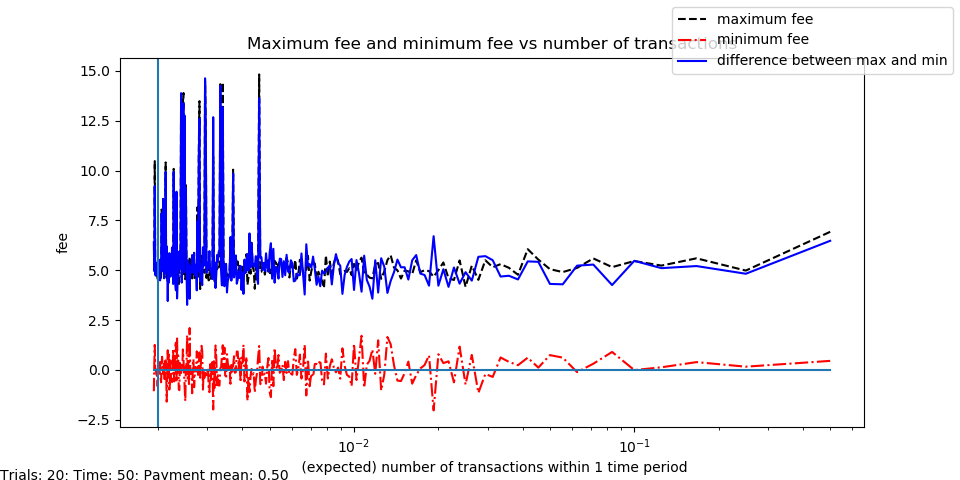
\includegraphics[scale=0.32]{figure/3n_f0.png}
    \end{center}
    \caption{Channel costs with respect to number of transactions}
    \label{figure_3Node4} 
    \floatfoot{As expected number of transactions within 1 time unit increases, when maximum fee is greater than minimum fee, it is more optimal to use the indirect channel. When maximum fee is less than minimum fee, and number of transactions is less than the vertical bound, it is more optimal to use on-chain transactions. After passing the vertical bound, Alice opens up her own channel with Charlie. }
\end{figure}
%%%%%%%%%%%%%%%% end figure %%%%%%%%%%%%%%%%%%%
%%%%%%%%%%%%%%%% begin figure %%%%%%%%%%%%%%%%%%%
\begin{figure}[t]
    \begin{center}
    \setlength{\unitlength}{0.012500in}%
    \includegraphics[scale=0.32]{figure/3n_f1.png}
    \end{center}
    \caption{Channel costs with respect to frequency}
    \label{figure_3Node5} 
    \floatfoot{Frequency refers to the amount of time between each transaction. As frequency gets smaller, the more transactions are sent during a time period. }
\end{figure}
%%%%%%%%%%%%%%%% end figure %%%%%%%%%%%%%%%%%%%
In figure 4, with payment size mean being $0.5$, we find that an agreement to the fee can be reached if the expected number of transactions within in time unit is 5. ($\lambda = 0.2$). As $\lambda$ decreases and the expected number of transactions increases, both maximum fee and the minimum fee increases at different rates, such that the two parties cannot find a mutually beneficial fee if the number of transactions exceeds 5. 

It is reasonable to make the conclusion that increasing $\lambda$ causes the fee to be lower, while increasing payment size causes the fee to increase. 

Also, note that the vertical line indicates the minimum $\lambda$ or maximum expected number of transactions for when Alice would prefer to make transactions outside of lightning. We calculated this line based on Lemma 0.1 from Clara's document "Asymptotic for Lightning Network" section 0.7. The interval between the vertical line and the intersection is the range of frequency that Alice would prefer to create a direct channel with Charlie instead of using indirect transfers or make on-chain transactions. 

We then generate a 3D model to further investigate the fee's behavior with respect to both payment size and frequency lambda. 

%%%%%%%%%%%%%%%%%%%%%%%%%%%%%%%%%%%%%%%%%%%%%%%%%%%%%%%%%%%%%%%%%%%%%%

\subsection{A 3D view with respect to size and frequency }
%%%%%%%%%%%%%%%%%%%%%%%%%%%%%%%%%%%%%%%%%%%%%%%%%%%%%%%%%%%%%%%%%%%%%%
%%%%%%%%%%%%%%%% begin figure %%%%%%%%%%%%%%%%%%%
\begin{figure}[t]
    \begin{center}
    \setlength{\unitlength}{0.012500in}%
    \includegraphics[scale=0.45]{figure/3n_pf_users.png}
    \end{center}
    \caption{The channel costs of each node}
    \label{figure_3Node6} 
    \floatfoot{In network 0, no transactions depend on the transferred payment, so there are no cost correlations. In network 1, only Alice is affected by the transferred payment has she creates a direct channel. In network 2, both Alice and Bob are affected by the indirect payments which is correlated with their channel costs. }
\end{figure}
%%%%%%%%%%%%%%%% end figure %%%%%%%%%%%%%%%%%%%

By looking at the cost of the channels in 3 different networks (fig 6), we observe that there is a relationship between frequency, size, and the cost of the channels in network 1 (for Alice) and network 2, while the indirect transaction doesn't exist in network 1 (for Bob) and network 0. 

To find the possible fees, we calculate the maximum and minimum fee bound. To be more specific, we find the difference between maximum and minimum fee, since a positive difference means that there exist a feasible fee bound, and a strictly negative difference means that there does not exist a feasible fee bound. 

In figure 7, we show the simulated result of such differences. Given a fixed frequency, the differences increase as payment size decreases. Given a fixed payment size, the differences increase as frequency increases, which we can interpret as the differences increases as the number of transactions within a time unit decreases. This means that it is easier to find a feasible fee when the payment is small, or when the number of transactions within a time unit is small. 

%%%%%%%%%%%%%%%%%%%%%%%%%%%%%%%%%%%%%%%%%%%%%%%%%%%%%%%%%%%%%%%%%%%%%%
%%%%%%%%%%%%%%%% begin figure %%%%%%%%%%%%%%%%%%%
\begin{figure}[t]
    \begin{center}
    \setlength{\unitlength}{0.012500in}%
    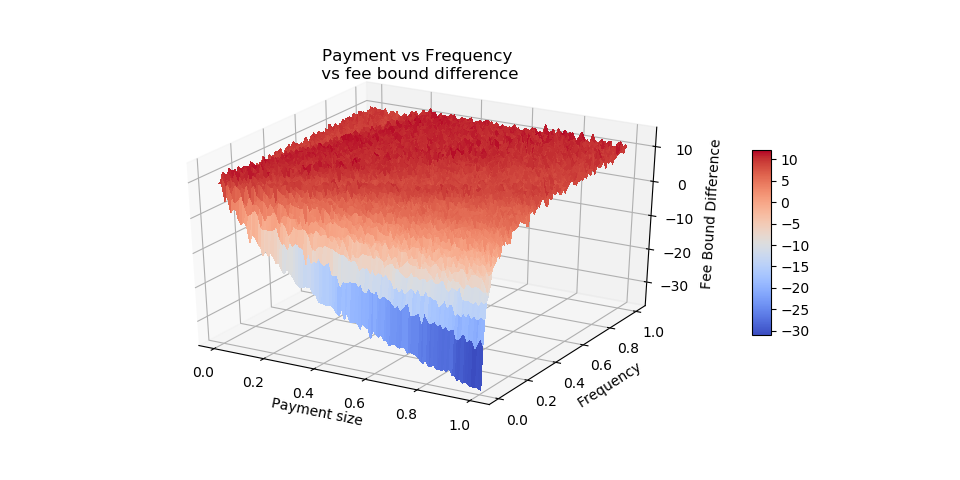
\includegraphics[scale=0.3]{figure/3node_pf.png}
    \end{center}
    \caption{Fee differences with respect to payment and frequency.}
    \label{figure_3Node7} 
    \floatfoot{For fee differences at less 0, the bound shows that the payment and frequency are feasible for indirect transactions, otherwise the bound is infeasible. A smaller payment will allow more indirect payments to route through the intermediate node during a time unit. }
\end{figure}
%%%%%%%%%%%%%%%% end figure %%%%%%%%%%%%%%%%%%%

A more direct way to view the differences is to see when it cross from positive to negative. Figure 8 shows the intercepts of the differences. Based on these points, we are able to locate the exact point at which larger payments or more frequent transactions become infeasible. This graph shows a more direct relationship between frequency and payment. A smaller payment will allow more indirect payments to route through the intermediate node during a time unit. 

%%%%%%%%%%%%%%%% begin figure %%%%%%%%%%%%%%%%%%%
\begin{figure}[t]
    \begin{center}
    \setlength{\unitlength}{0.012500in}%
    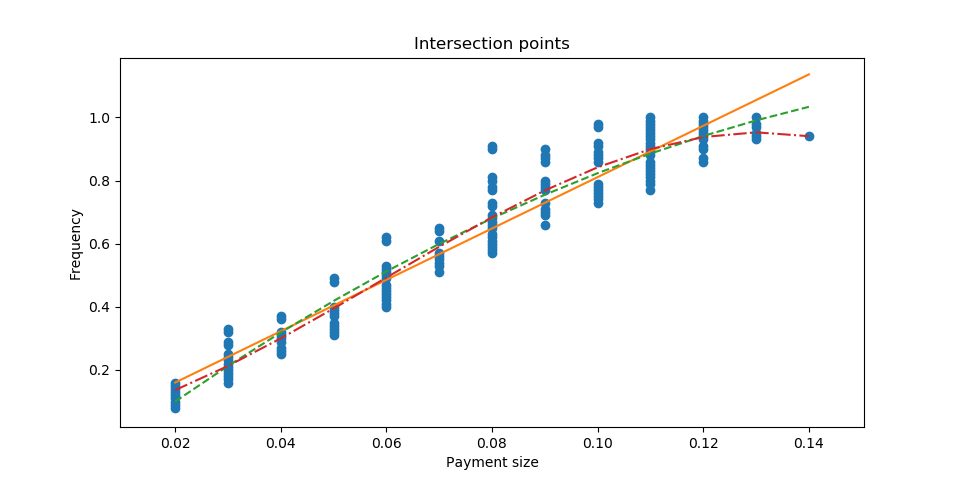
\includegraphics[scale=0.3]{figure/3node_pf_inter.png}
    \end{center}
    \caption{Intersection of payment and frequency where maximum and minimum fee equates each other .}
    \label{figure_3Node8} 
    \floatfoot{For all the points, maximum fee equates minimum fee. The best fit line of order 1, 2, and 3 attempts to learn their relationship.}
    \end{figure}
%%%%%%%%%%%%%%%% end figure %%%%%%%%%%%%%%%%%%%


\subsection{Setup 1}
with a more applicable example, let's flip the payment between Bob and Charlie. This example reassemble the scenario in which Bob is a company, while Alice and Charlie are both Bob's consumers, and Alice wants to send some payment to Charlie. An instance for this network is if Bob is a coffee shop, and Alice and Charlie buys coffee from Bob regularly, while Alice pays Charlie occasionally for something else. 

We show the 3D view for analyzing how does the fee differences behave under the new setup of the payments.  

%%%%%%%%%%%%%%%% begin figure %%%%%%%%%%%%%%%%%%%
\begin{figure}[t]
    \begin{center}
    \setlength{\unitlength}{0.012500in}%
    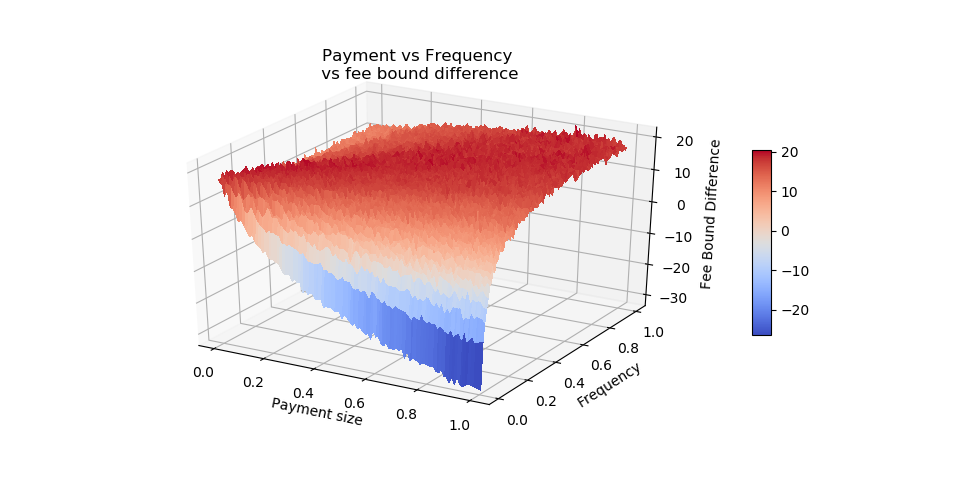
\includegraphics[scale=0.3]{figure/3node_pfOppo.png}
    \end{center}
    \caption{feasible fee bounds in opposite direction}
    \label{figure_3Node11} 
    \floatfoot{For fee differences at less 0, the bound shows that the payment and frequency are feasible for indirect transactions, otherwise the bound is infeasible. A smaller payment will allow more indirect payments to route through the intermediate node during a time unit. }
    \end{figure}
%%%%%%%%%%%%%%%% end figure %%%%%%%%%%%%%%%%%%%

We use the intersections to find where the bounds becomes infeasible or feasible. 


%%%%%%%%%%%%%%%% begin figure %%%%%%%%%%%%%%%%%%%
\begin{figure}[t]
    \begin{center}
    \setlength{\unitlength}{0.012500in}%
    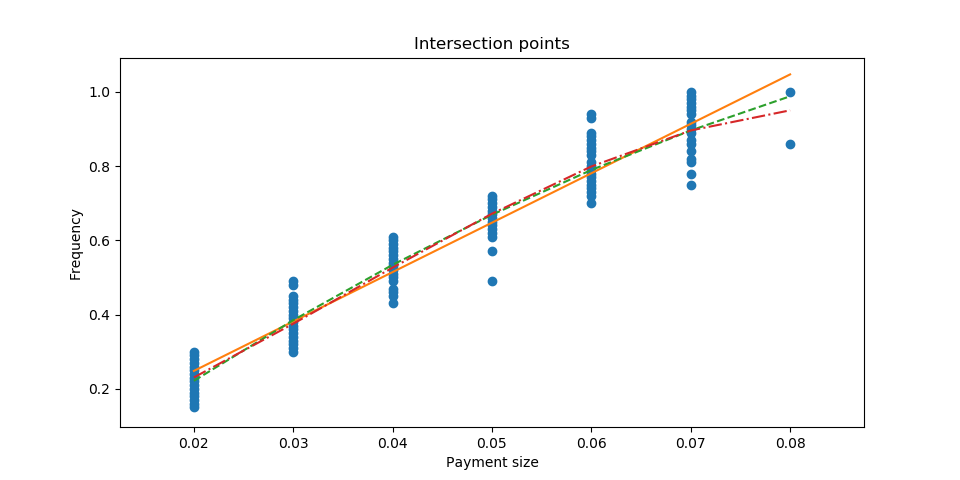
\includegraphics[scale=0.3]{figure/3node_pf_interOppo.png}
    \end{center}
    \caption{intersection of fee bounds in opposite direction}
    \label{figure_3Node12} 
    \floatfoot{For all the points, maximum fee equates minimum fee. The best fit line of order 1, 2, and 3 attempts to learn their relationship.}
    \end{figure}
%%%%%%%%%%%%%%%% end figure %%%%%%%%%%%%%%%%%%%

Comparing figure 8 with figure 10, intersection best fit lin for opposite direction setup has a steeper slope for different orders of best fit line, thus the feasible interval of the differences are larger, such that more specifications of the routed payment can transfer through the opposite direction's setup. 

\subsection{Discussion}
As payment size increase or the rate of transactions sent from Alice to Charlie, Bob's channel balances changes with higher velocity, thus possibly making Bob to renew the channels more often. This intuition can be seen through the simulation. 

The simulation results suggest that higher amount of payments and larger size of payments causes maximum fee to decrease and minimum fee to increase, leading to smaller or even infeasible fee bound. however, once payment sizes are small enough or the frequency is large enough, indirect transfers are encouraged instead of building direct channels if we only look at channel costs. While we are looking at the three-node structure, we are overlooking many other factors, such as the value of a centralized node, incentive to balance channel capacities, inconsistent payments, etc. Despite the overlooked extra specifications, the model shows clear criteria for the fee bound feasibility based on payment size and frequency.

When comparing two types of setups of the same network, we find that if the indirect payment goes against the direction of some payments on the route of transfers, the feasible interval of the differences are larger. We can explain this change as if Bob is extra incentivized to serve as an intermediate node for rebalancing the channels. If the payments are going against the direction of Bob's regular payments, Bob may update his channels less often, thus decreasing the cost to maintain the channel. When the payments are significant enough, Bob might be incentivized to pay Alice for such indirect transfers. Naturally, we further investigate the possibility of negative minimum fee. 



\subsection{Setup 2}
Say that the Bob transfers to Alice, and Charlie transfers to Bob, then Alice's payment to Charlie goes against the regular transactions. Intuitively, Bob can rebalance his channel using Alice's payment to Charlie. Thus we setup such a network to investigate if Bob will be incentivized enough to pay Alice to route through him, which can be seen if there exist negative minimum fees.

%%%%%%%%%%%%%%%% begin figure %%%%%%%%%%%%%%%%%%%
\begin{figure}[t]
    \begin{center}
    \setlength{\unitlength}{0.012500in}%
    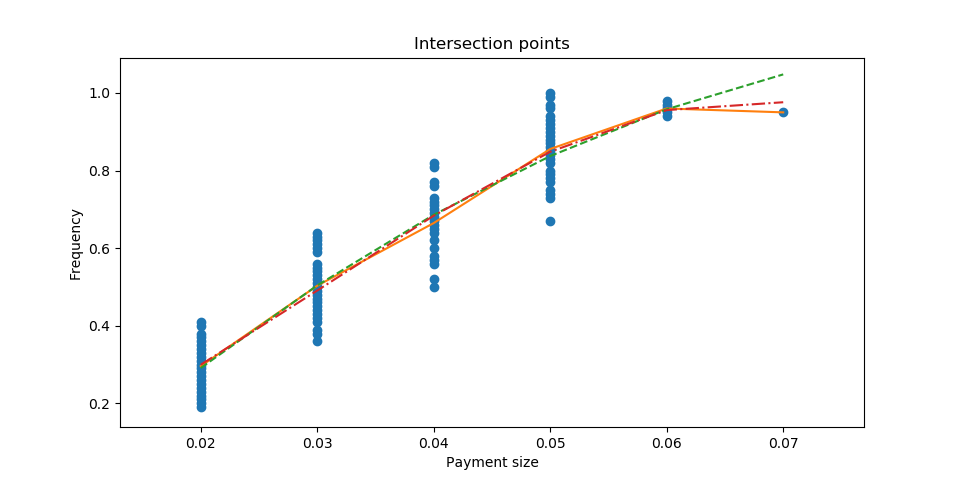
\includegraphics[scale=0.3]{figure/3node_pf_interOppo2.png}
    \end{center}
    \caption{feasible fee bounds in opposite direction}
    \label{figure_3Node11} 
    \floatfoot{The minimum fee varies across payment and frequency, but seem positive throughout. }
    \end{figure}
%%%%%%%%%%%%%%%% end figure %%%%%%%%%%%%%%%%%%%

First we show the intersection points, which has a lower slope than the other two intersection point graphs. This can be interpreted as more payments and bigger payments can go through indirectly. 

To find out if it is possible to have a negative transaction fee, we focus on Bob's costs to see if Bob will, at any point, has a lower cost to maintain the costs, thus has a negative minimum transaction fee. 

%%%%%%%%%%%%%%%% begin figure %%%%%%%%%%%%%%%%%%%
\begin{figure}[t]
    \begin{center}
    \setlength{\unitlength}{0.012500in}%
    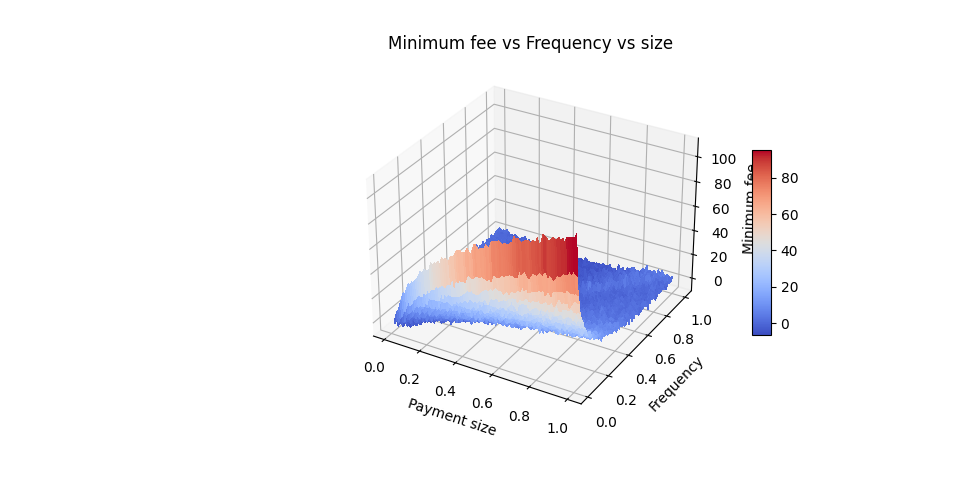
\includegraphics[scale=0.55]{figure/3node_pfMinfee2.png}
    \end{center}
    \caption{feasible fee bounds in opposite direction}
    \label{figure_3Node11} 
    \floatfoot{The minimum fee varies across payment and frequency, but seem positive throughout. }
    \end{figure}
%%%%%%%%%%%%%%%% end figure %%%%%%%%%%%%%%%%%%%

Through figure 11, we see that the minimum of the minimum fee stays positive. It is important to either test out more combination of size, frequency, or network configurations to find out if it is possible to have a negative fee, while this particular example was not able to provide such an instance. 


%%%%%%%%%%%%%%%%%%%%%%%%%%%%%%%%%%%%%%%%%%%%%%%%%%%%%%%%%%%%%%%%%%%%%%
\subsection{Theory}
%%%%%%%%%%%%%%%%%%%%%%%%%%%%%%%%%%%%%%%%%%%%%%%%%%%%%%%%%%%%%%%%%%%%%%
Building on top of Clara's documents, we attempt to find the exquation for fee bounds. 

\begin{itemize}
    \item $p$ - size of the transferred payment
    \item $f$ - rate of the transferred payment (expected number of payments per time unit)
    \item $B$ - price of on-chain transaction, assumed to be $5$
    \item $r$ - constant rate of interest, assumed to be $0.01$
    \item $P,F$ - size and rate of other payments, assumed to be $1$
\end{itemize}


\subsubsection{Interest return}

Let $\tau$ be an random variable of exponential distribution with parameter $\alpha$. $\tau$ indicates the time a channel is used, in our simulation, it is set to be a constant of 50. We assume that Bob saves an extra $p$ in the account to ensure the success of transactions. 

By storing $\frac{c}{e^{r\tau}}$ in the bank at time $t=0$, the balance grow to $c$ at time $t=\tau$. So the cost for Bob to store an extra $p$ in the channel for transfers, the opportunity cost is estimated to be 
\begin{equation}
    I_\tau = p-pe^{-r\tau}
\end{equation}

% Then the expected interest return of a channel is 
% \begin{equation}
%     I(\alpha) = E[I_\alpha] = p-pE[e^{-r\tau}] = p-p\frac{\alpha}{\alpha + r}
% \end{equation}

% Assuming that Bob charges a total of $P$ for the entire time the channel is used, then the transaction fee Bob gets is simply 
% \begin{equation}
%     T_{\tau}= P \cdot e^{-r\tau}
% \end{equation}

\subsubsection{Three node network setup 0}

Recall the network setup of 3 nodes first direction. We first find the optimal sizes of the channel using equation $m_{1} = (B\lambda/r)^{1/2}$ and $m_{2}=(2B\lambda / r)^{1/3}$, and we use $m_{1}$ for the one-directional payments, which is what we are focused on.

We plug in the size for the expected cost of the channel, with the assumptions we made for the network setup. 
%%%%%%%%%%%%%%%%%%%%%%%%%%%%%%%%%%%%%%%%%%%%%%%%%%%%%%%%%%%%%%%%%%%%%%
%%%%%%%%%%%%%%% begin table   %%%%%%%%%%%%%%%%%%%%%%%%%%
\begin{table}[t]
\caption{Estimated cost of channels}
\begin{center}
\label{table_ASME}
\begin{tabular}{c l l}
& &  \\ % put some space after the caption
\hline
Network & Bob & Alice + Charlie \\
\hline
N0 & $(\frac{2BP}{rF})^{1/2}$ & $=\text{Bob  N0}$ \\
N1 & $(\frac{2BP}{rF})^{1/2}$ & $(\frac{2B}{r})^{1/2}((\frac{P}{F})^{1/2}+(\frac{p}{f})^{1/2})$\\
N2-0 & $(\frac{2B(\frac{P}{F}+\frac{p}{f})}{r})^{1/2}$& $=\text{Bob  N2-0}$ \\
N2-1 & $\frac{1}{2}(\frac{2B(\frac{P}{F}+\frac{p}{f})}{r})^{1/2}$\\
& $+\frac{1}{2}(\frac{2B(\frac{P}{F}-\frac{p}{f})}{r})^{1/3}$& $=\text{Bob  N2-1}$ \\
N2-2 & $(\frac{2B(\frac{P}{F}-\frac{p}{f})}{r})^{1/3}$& $=\text{Bob  N2-2}$ \\
% \hline 
% & Bob' & AC' \\
% \hline 
% N2 & $2(\frac{2B(\frac{P}{F}+\frac{p}{f})}{r})^{1/2}-(\frac{2BP}{rF})^{1/2}$& $(\frac{2BP}{rF})^{1/2}$ \\
\hline
\end{tabular}
\end{center}
\end{table}
%%%%%%%%%%%%%%%% end table %%%%%%%%%%%%%%%%%%% 
%%%%%%%%%%%%%%%%%%%%%%%%%%%%%%%%%%%%%%%%%%%%%%%%%%%%%%%%%%%%%%%%%%%%%%

With the table, we can calculate, with our implementation of service fees, $b2'=2(\frac{2B(\frac{P}{F}+\frac{p}{f})}{r})^{1/2}-(\frac{2BP}{rF})^{1/2}$, and $a2'=(\frac{2BP}{rF})^{1/2}$, so
\begin{align}
    max\;fee &= a1-a0=(\frac{2B}{r})^{1/2}(\frac{p}{f})^{1/2}\\
    min\;fee &= b2'-b0=2(\frac{2B(\frac{P}{F}+\frac{p}{f})}{r})^{1/2}-2(\frac{2BP}{rF})^{1/2}
\end{align}
Recall that Bob's opportunity cost is
\begin{align}
    I(\tau)= p-pe^{-r\tau}=p-pe^{-0.5}
\end{align}
The setup has a sepcification of a constant time in the setup, but let us estimate the cost of the channel with near $0 $ time, such that $p-pe^{-r\tau}\rightarrow 0 $ as $\tau \rightarrow 0$, so the opportunity cost becomes 0. \\
In order to find the intersection point, we find where maximum fee equates minimum fee.
\begin{align}
    (\frac{2B}{r})^{1/2}(\frac{p}{f})^{1/2} =  2(\frac{2B(\frac{P}{F}+\frac{p}{f})}{r})^{1/2}-2(\frac{2BP}{rF})^{1/2}
\end{align}
Since we have used the parameters $B=5$, $r=0.01$, and $F=P=1$, we plug it in to simplify the approximation of the intersection.
\begin{align}
    (\frac{p}{f})^{1/2} =  2(1+\frac{p}{f})^{1/2}-2 \Rightarrow \frac{p}{f}=\frac{16}{9}
\end{align}

Note that the constants do not match our result, but the relationship does appear to be positive of each other. 

\subsubsection{Three node network setup 1}

With similar calculation, we get that without splitting the additional channel costs, 
\begin{align}
    b2'& = (\frac{2B(\frac{P}{F}+\frac{p}{f})}{r})^{1/2}+(\frac{2B(\frac{P}{F}-\frac{p}{f})}{r})^{1/3}-(\frac{2BP}{rF})^{1/2} 
\end{align}
and other costs stays the same. The difference with the costs mainly occurs because the channel between Bob and Charlie becomes bidirectional due to the opposite direction of payments. 

Thus to find the intersection, we set minimum fee and maximum fee equal to each other and get
\begin{align}
    &(1000(1-\frac{p}{f}))^{1/3}=1000^{1/2} \\
    \Rightarrow & (1-\frac{p}{f})^{1/3}=\sqrt{10}
\end{align}


\subsubsection{Three node network setup 2}

With similar calculation, we get that without splitting the additional channel costs, 
\begin{align}
    b2'& = 2(\frac{2B(\frac{P}{F}-\frac{p}{f})}{r})^{1/3}-(\frac{2BP}{rF})^{1/2} 
\end{align}
and other costs stays the same. The difference with the costs mainly occurs because Bob's channel become bidirectional due to the opposite direction of payments. 

Thus to find the intersection, we set minimum fee and maximum fee equal to each other and get
\begin{align}
    & 2(1-\frac{p}{f})^{1/3}/1000^{1/6} =2+(\frac{p}{f})^{1/2}
\end{align}



%%%%%%%%%%%%%%%%%%%%%%%%%%%%%%%%%%%%%%%%%%%%%%%%%%%%%%%%%%%%%%%%%%%%%%


\subsection{Comparison and discussion}

%%%%%%%%%%%%%%%% begin figure %%%%%%%%%%%%%%%%%%%
\begin{figure}[t]
    \begin{center}
    \setlength{\unitlength}{0.012500in}%
    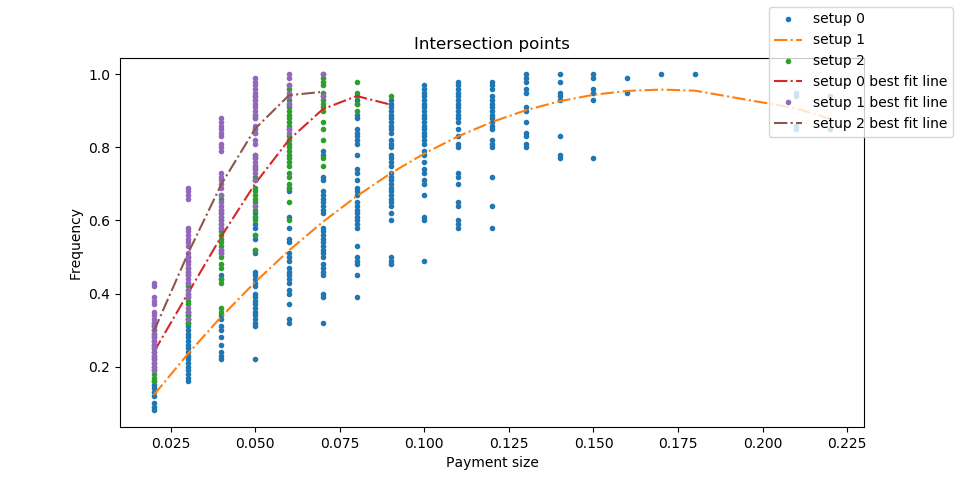
\includegraphics[scale=0.35]{figure/compareInt.png}
    \end{center}
    \caption{Compare 3 node structure 1}
    \label{figure_4Node1} 
    \end{figure}
%%%%%%%%%%%%%%%% end figure %%%%%%%%%%%%%%%%%%%

Comparing the three intersection point graphs, we have shown that setup 2 has the deepest slope, thus allowing more combinations of payments to go through. However, due to the dip at the end, we increase the range of the payments and frequency to find the behavior of intersection points for all three setups. 

%%%%%%%%%%%%%%%% begin figure %%%%%%%%%%%%%%%%%%%
\begin{figure}[t]
    \begin{center}
    \setlength{\unitlength}{0.012500in}%
    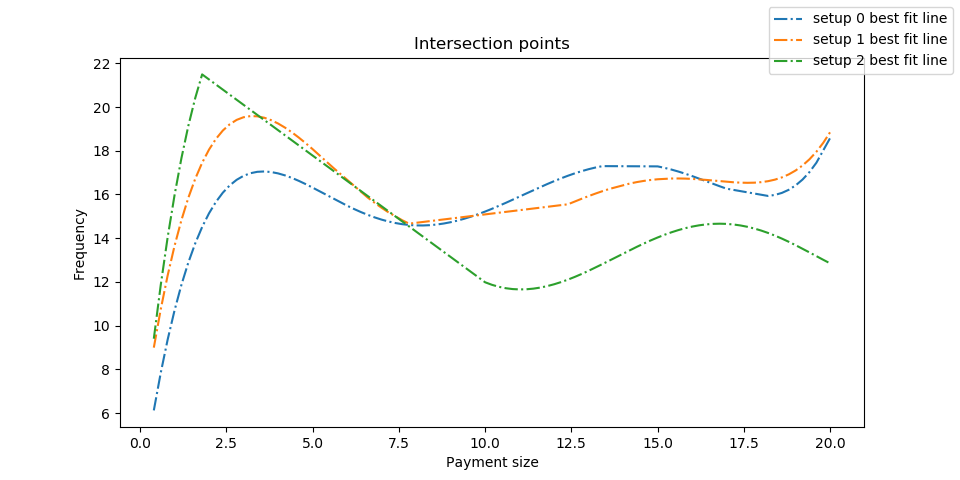
\includegraphics[scale=0.35]{figure/compareInt_large.png}
    \end{center}
    \caption{Compare 3 node structure 1}
    \label{figure_4Node1} 
    \end{figure}
%%%%%%%%%%%%%%%% end figure %%%%%%%%%%%%%%%%%%%

It is interesting to see that setup 2 eventually become the least incentivizing setup after payment size grows above 1. This could be explained by the increasing in cost of bidirectional channels. While setup 0 only has unidirectional channels, setup 2 becomes more expensive to maintain as the channel sizes are increased significantly. 


%%%%%%%%%%%%%%%%%%%%%%%%%%%%%%%%%%%%%%%%%%%%%%%%%%%%%%%%%%%%%%%%%%%%%%


\section{Four Node Structure 0}
%%%%%%%%%%%%%%%% begin figure %%%%%%%%%%%%%%%%%%%
\begin{figure}[t]
    \begin{center}
    \setlength{\unitlength}{0.012500in}%
    \includegraphics[scale=0.65]{figure/4nodeDiagram0.jpg}
    \end{center}
    \caption{A 4 node network, structure 0.}
    \label{figure_4Node1} 
    \end{figure}
%%%%%%%%%%%%%%%% end figure %%%%%%%%%%%%%%%%%%%

After analyzing the simplest case, we extend the analysis to 4 nodes structures. The first structure of the 4 node network analysis is the comparison between indirect transfer of a star, and creating a direct channel between the two leaf nodes, thus creating a triangular cycle. A real life example of what this example would be useful is we let Bob be a streaming service, while A, C, D are costumers. A wants to pay D and has the option to route the payment through Bob, or create a direct channel. 

This is exceedingly similar to the 3 node structure, thus we expect a similar result. 

Bob is the intermediate node, and Alice, Donna, and Charlie are end nodes. We recognize that Charlie is not affected by A's payment to Donna, and whether to include Charlie does not affect our results. We find each party's cost of channels in these two networks. 

By doing so, we find the fee bounds based on maximum or minimum fee charges, following the calculations from the previous section to get the intersections. 

% %%%%%%%%%%%%%%%% begin figure %%%%%%%%%%%%%%%%%%%
% \begin{figure}[t]
%     \begin{center}
%     \setlength{\unitlength}{0.012500in}%
%     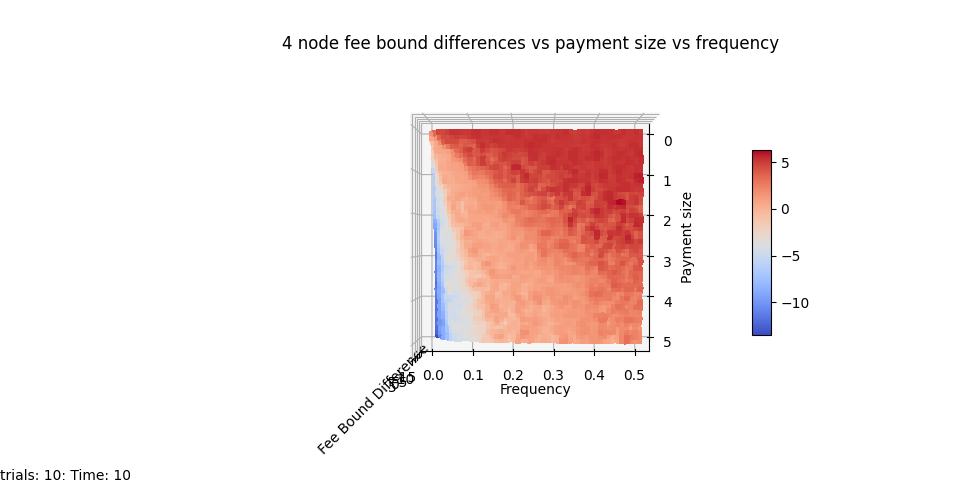
\includegraphics[scale=0.3]{figure/4node_pf0.png}
%     \end{center}
%     \caption{A 4 node network, structure 0. Feasiblity of fee bound.}
%     \label{figure_4Node2} 
%     \end{figure}
% %%%%%%%%%%%%%%%% end figure %%%%%%%%%%%%%%%%%%%

%%%%%%%%%%%%%%%% begin figure %%%%%%%%%%%%%%%%%%%
\begin{figure}[t]
    \begin{center}
    \setlength{\unitlength}{0.012500in}%
    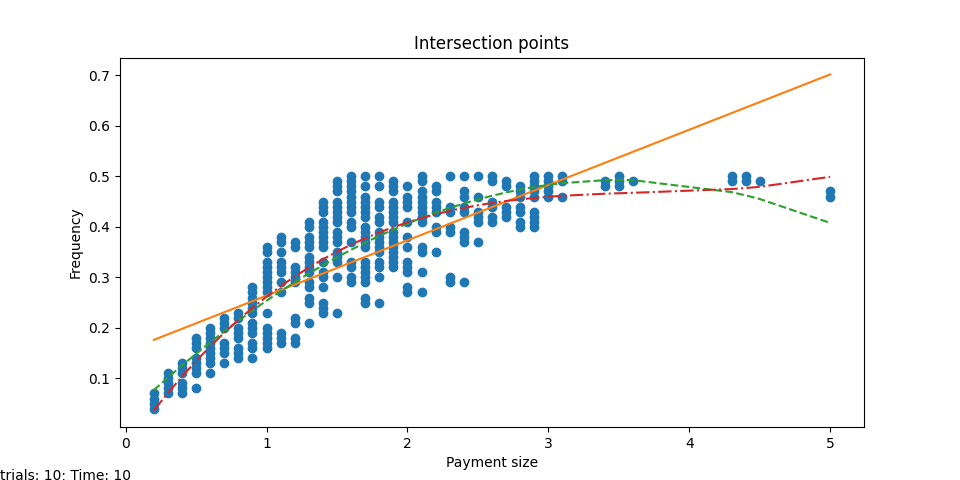
\includegraphics[scale=0.3]{figure/4node_pf_inter0.png}
    \end{center}
    \caption{A 4 node network, structure 0. Intersection of feasibility on payment and frequency.}
    \label{figure_4Node3} 
    \floatfoot{Points where maximum fee equates minimum fee. Best line of fit of order 1, 2, 3 suggests a weak positive relationship between frequency and size}
    \end{figure}
%%%%%%%%%%%%%%%% end figure %%%%%%%%%%%%%%%%%%%
Through figure 12, we find that the best fit line of order 1 and 3 suggested a non-linear positive relationship between payment size and frequency, similar to that of 3 node structures. It is possible that we can prove the four node can be reduced to a three node structure. 


%%%%%%%%%%%%%%%%%%%%%%%%%%%%%%%%%%%%%%%%%%%%%%%%%%%%%%%%%%%%%%%%%%%%%%


%%%%%%%%%%%%%%%%%%%%%%%%%%%%%%%%%%%%%%%%%%%%%%%%%%%%%%%%%%%%%%%%%%%%%%
\section{Four Node Structure 1}
%%%%%%%%%%%%%%%% begin figure %%%%%%%%%%%%%%%%%%%
\begin{figure}[t]
    \begin{center}
    \setlength{\unitlength}{0.012500in}%
    \includegraphics[scale=0.65]{figure/4nodeDiagram1.jpg}
    \end{center}
    \caption{A 4 node network, structure 1.}
    \label{figure_4Node4} 
    \end{figure}
%%%%%%%%%%%%%%%% end figure %%%%%%%%%%%%%%%%%%%

Now, say that Alice not only want to send tokens to Donna, but also Charlie. Will Alice still use Bob's service? The second structure of the 4 node network analysis is the comparison between indirect transfer of a star, and creating a direct channel between the leaf nodes, thus creating 2 triangular cycles. 

Bob is the intermediate nodes, and Alice, Charlie and Donna be the end nodes, represented by Alice. Charlie's transactions are not affected by the change in the network. We find each party's cost of channels in these two networks. 

By doing so, we find the fee bounds based on maximum or minimum fee charges. 

Observing figure 14, we find that the best fit lines look similar to that of figure 12, which means that we can possibly reduce structure 1 to structure 0. Furthermore, it might imply that we can then reduce structure 1 to a three node structure.  
% %%%%%%%%%%%%%%%% begin figure %%%%%%%%%%%%%%%%%%%
% \begin{figure}[t]
%     \begin{center}
%     \setlength{\unitlength}{0.012500in}%
%     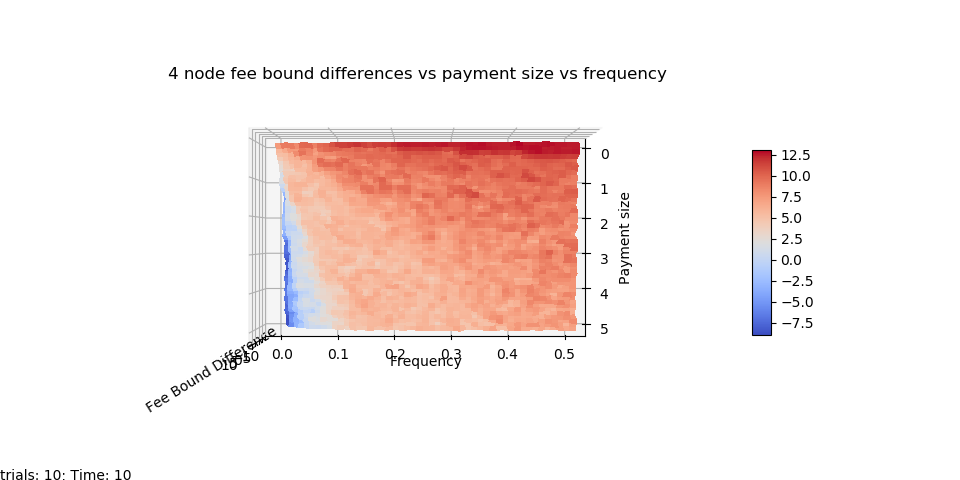
\includegraphics[scale=0.3]{figure/4node_pf1.png}
%     \end{center}
%     \caption{A 4 node network, structure 1. Feasibility of the fee bound.}
%     \label{figure_4Node5} 
%     \end{figure}
% %%%%%%%%%%%%%%%% end figure %%%%%%%%%%%%%%%%%%%


%%%%%%%%%%%%%%%% begin figure %%%%%%%%%%%%%%%%%%%
\begin{figure}[t]
    \begin{center}
    \setlength{\unitlength}{0.012500in}%
    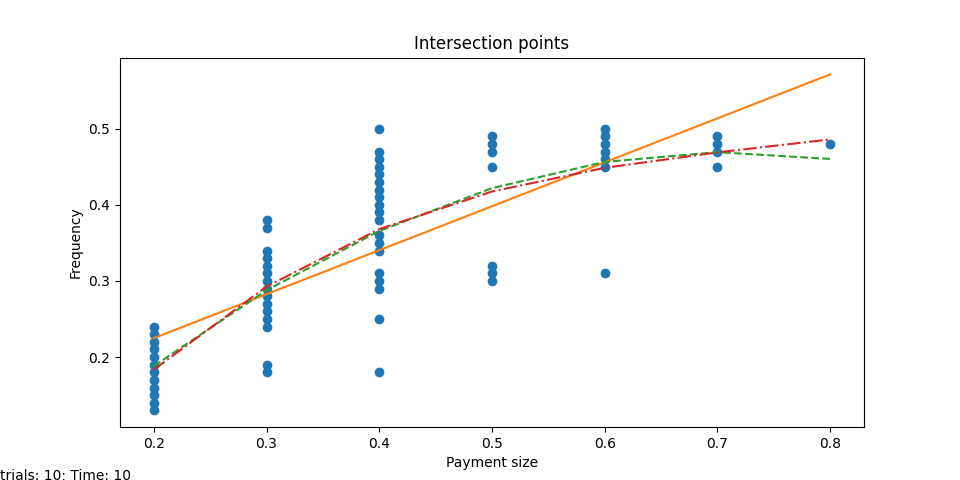
\includegraphics[scale=0.3]{figure/4node_pf_inter1.png}
    \end{center}
    \caption{A 4 node network, structure 1. Intersection of feasibility on payment and frequency.}
    \label{figure_4Node6} 
    \floatfoot{Points where maximum fee equates minimum fee. Best line of fit of order 1, 2, 3 suggests a weak positive relationship between frequency and size}
    \end{figure}
%%%%%%%%%%%%%%%% end figure %%%%%%%%%%%%%%%%%%%



%%%%%%%%%%%%%%%%%%%%%%%%%%%%%%%%%%%%%%%%%%%%%%%%%%%%%%%%%%%%%%%%%%%%%%



%%%%%%%%%%%%%%%%%%%%%%%%%%%%%%%%%%%%%%%%%%%%%%%%%%%%%%%%%%%%%%%%%%%%%%
\section{Four Node Structure 2}
%%%%%%%%%%%%%%%%%%%%%%%%%%%%%%%%%%%%%%%%%%%%%%%%%%%%%%%%%%%%%%%%%%%%%%
%%%%%%%%%%%%%%%% begin figure %%%%%%%%%%%%%%%%%%%
\begin{figure}[t]
    \begin{center}
    \setlength{\unitlength}{0.012500in}%
    \includegraphics[scale=0.65]{figure/4nodeDiagram2.jpg}
    \end{center}
    \caption{A 4 node network, structure 2.}
    \label{figure_4Node7} 
\end{figure}
%%%%%%%%%%%%%%%% end figure %%%%%%%%%%%%%%%%%%%
The second structure of the 4 node network analysis is the comparison between indirect transfer of a chain of 4 nodes, and creating a direct channel between the beginning and the end of the chain, thus creating a cycle. 

We let Bob and Charlie be intermediate nodes, represented by Bob, and Alice and Donna be the end nodes, represented by Alice. We find each party's cost of channels in these two networks, and the fee bounds based on maximum or minimum fee charges. 

% %%%%%%%%%%%%%%%% begin figure %%%%%%%%%%%%%%%%%%%
% \begin{figure}[t]
%     \begin{center}
%     \setlength{\unitlength}{0.012500in}%
%     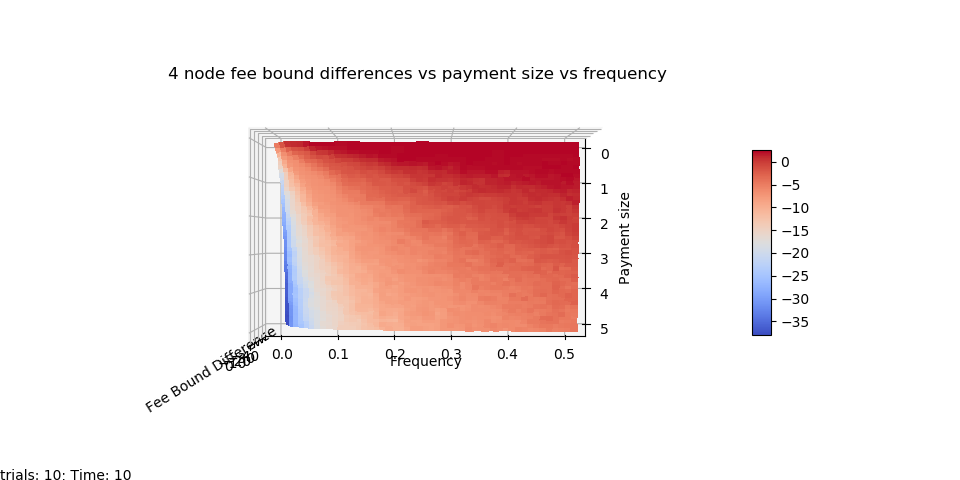
\includegraphics[scale=0.3]{figure/4node_pf2.png}
%     \end{center}
%     \caption{A 4 node network, fee bound differences (feasibility).}
%     \label{figure_4Node8} 
%     \end{figure}
% %%%%%%%%%%%%%%%% end figure %%%%%%%%%%%%%%%%%%%

%%%%%%%%%%%%%%%% begin figure %%%%%%%%%%%%%%%%%%%
\begin{figure}[t]
    \begin{center}
    \setlength{\unitlength}{0.012500in}%
    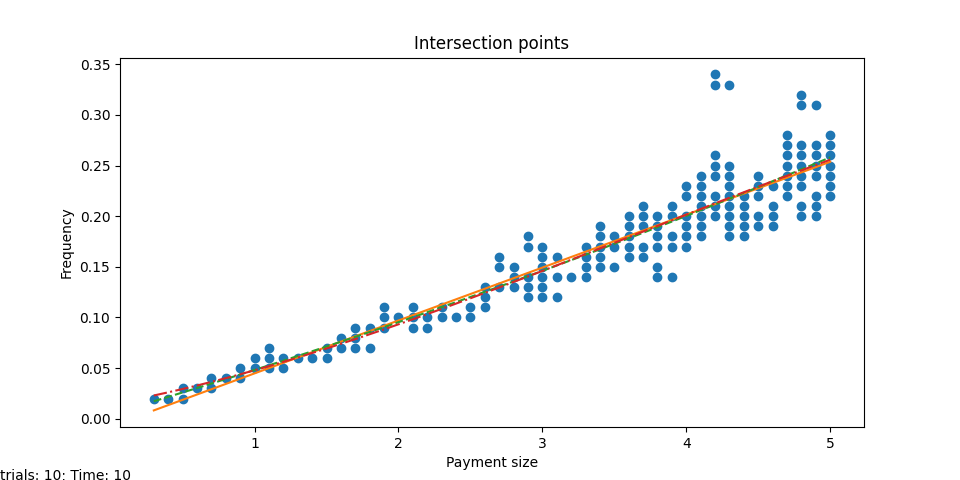
\includegraphics[scale=0.3]{figure/4node_pf_inter2.png}
    \end{center}
    \caption{A 4 node network, intersection of feasibility on payment and frequency.}
    \label{figure_4Node9} 
    \floatfoot{Points where maximum fee equates minimum fee. Best line of fit of order 1, 2, 3 suggests a weak positive relationship between frequency and size}
    \end{figure}
%%%%%%%%%%%%%%%% end figure %%%%%%%%%%%%%%%%%%%

In structure 16, the best fit lines reassemble 3 node structures. This means the intermediate nodes, although with a longer route, can be reduced into 1 single intermediate node if we treat their total costs as of one node. This could allow us to reduce structure 2 into a three node structure again. These reductions require further proofs. 

\subsection{Comparison}

Structure 0 and structure 1 are comparable since they have the same payments, with one extra indirect payment from Alice to Charlie. By comparing the two structures, we can observe how additional indirect payment affect the intermediate node Bob. 

In structure 1, Bob is the central node that connects Alice, Charlie, and Donna. Alice sends a indirect payment through Bob to Donna. In structure 2, Alice sends an additional payment through Bob to Charlie. By observing figure 12 and figure 15, we find that the shape of points in figure 15 are significantly different from that of figure 12. While the best fit line in 12 seems more linear, the best fit line in 15 does not appear linear. Thus, we try to do more analysis on the points. Note that the case of Alice only sending payments to Charlie is identical with Alice only sending payments to Donna. 

4 node structure 2 can be easily compared with 3 node structure direction 0, since in the 4 node structure, the intermediate node can be combined to one node. If we look at their best fit line of the intersection graph, both suggests a rather linear relationship between frequency and size. 



%%%%%%%%%%%%%%%%%%%%%%%%%%%%%%%%%%%%%%%%%%%%%%%%%%%%%%%%%%%%%%%%%%%%%%

\section{Conclusion}
By running simulations, we find that smaller payments or less frequent payments are encouraged to be traded indirectly. The intersection plots shows that each payment or frequency requirement provides a bound towards the other, in order to make indirect transactions. 

There are a lot of possibility for further investigation, such as observing the intersection points' behavior near 0 of size or frequency, the possibility of a negative minimum fee, reduction of larger networks to three node networks, build transaction fee based on single payments and of each intermediate node instead of the total fee.





\end{document}
